\section{Prototipado}

Figma es una herramienta muy potente de diseño que permite la creación de prototipos
digitales altamente interactivos. Por ello, hemos empleado esta herramienta para poder
prototipar nuestras interfaces desarrolladas en el hito anterior, además de mejorarlas
aplicando aquellos cambios que se han considerado necesarios. Estos cambios serán explicados
en esta sección, además de detallar también los principios de diseño que aparecen en cada
una de las interfaces.

\subsection{Inicio}

La pantalla principal de nuestra aplicación (figura \ref{fig:it1_inicio}), como ya detallamos anteriormente, va a ser la de búsqueda,
en la que, a diferencia de lo planteado en el hito anterior, cualquier usuario va a poder realizar la
comparación de viajes (aunque no pueda finalizar sin tener que iniciar sesión o crearse una cuenta). Otro
de los cambios que además se ha realizado es ofrecer la posibilidad a los usuarios que no se hayan registrado
como discapacitados de poder buscar viajes accesibles sin tener que aplicar el filtro en la siguiente página
(el comparador). Sin embargo, a pesar de estos cambios, la esencia de la ventana es la misma, se mantiene la
barra de búsqueda con todas las opciones que se pedían anteriormente (el origen, el destino, la fecha de ida,
la fecha de vuelta y el número de asientos) y para completar se muestran las mejores ofertas en forma de
tarjetas para que el usuario vea de forma mucho más visual toda la información que ahí se expone. En cuanto a
los patrones y principios que se han seguido para esta pantalla, son los siguientes:

\begin{itemize}
    \item \textbf{Principio de proximidad.} Todos los campos requeridos para realizar una búsqueda se encuentran
        cercanos entre sí, además de encuadrados bajo un marco, lo que indica al usuario que todo el contenido
        solicitado es necesario para comenzar una búsqueda de transportes. Relacionado a ello, aplica la Ley de
        Fitts (la distancia que tiene que ser recorrida para moverse de un campo a otro es muy pequeña).
    \item \textbf{Consistencia interna.} Las distintas tarjetas que se presentan para mostrar las ofertas de la
        aplicación en la página de inicio guardan y muestran la misma cantidad de información: el logo de la compañía
        que lo opera, la fecha del viaje, el precio, las horas de salida y llegada y las estaciones. También presenta
        consistencia en cuanto a la forma de la tarjeta y los colores que se utilizan.
    \item \textbf{Consistencia externa.} Al igual que en la gran mayoría de las aplicaciones, cuando el usuario tiene la sesión
        iniciada en la página, puede acceder a su perfil pulsando sobre el botón de usuario situado en la esquina
        superior derecha.
    \item \textbf{Principio de visibilidad.} Del mismo modo que en el caso anterior, puede consultarse el estado en el que
        se encuentra la aplicación si en la esquina superior derecha te sale la opción de iniciar sesión o de
        registrarse (sesión no iniciada) o el icono del perfil (sesión iniciada).
\end{itemize}

\begin{figure}[H]
    \centering
    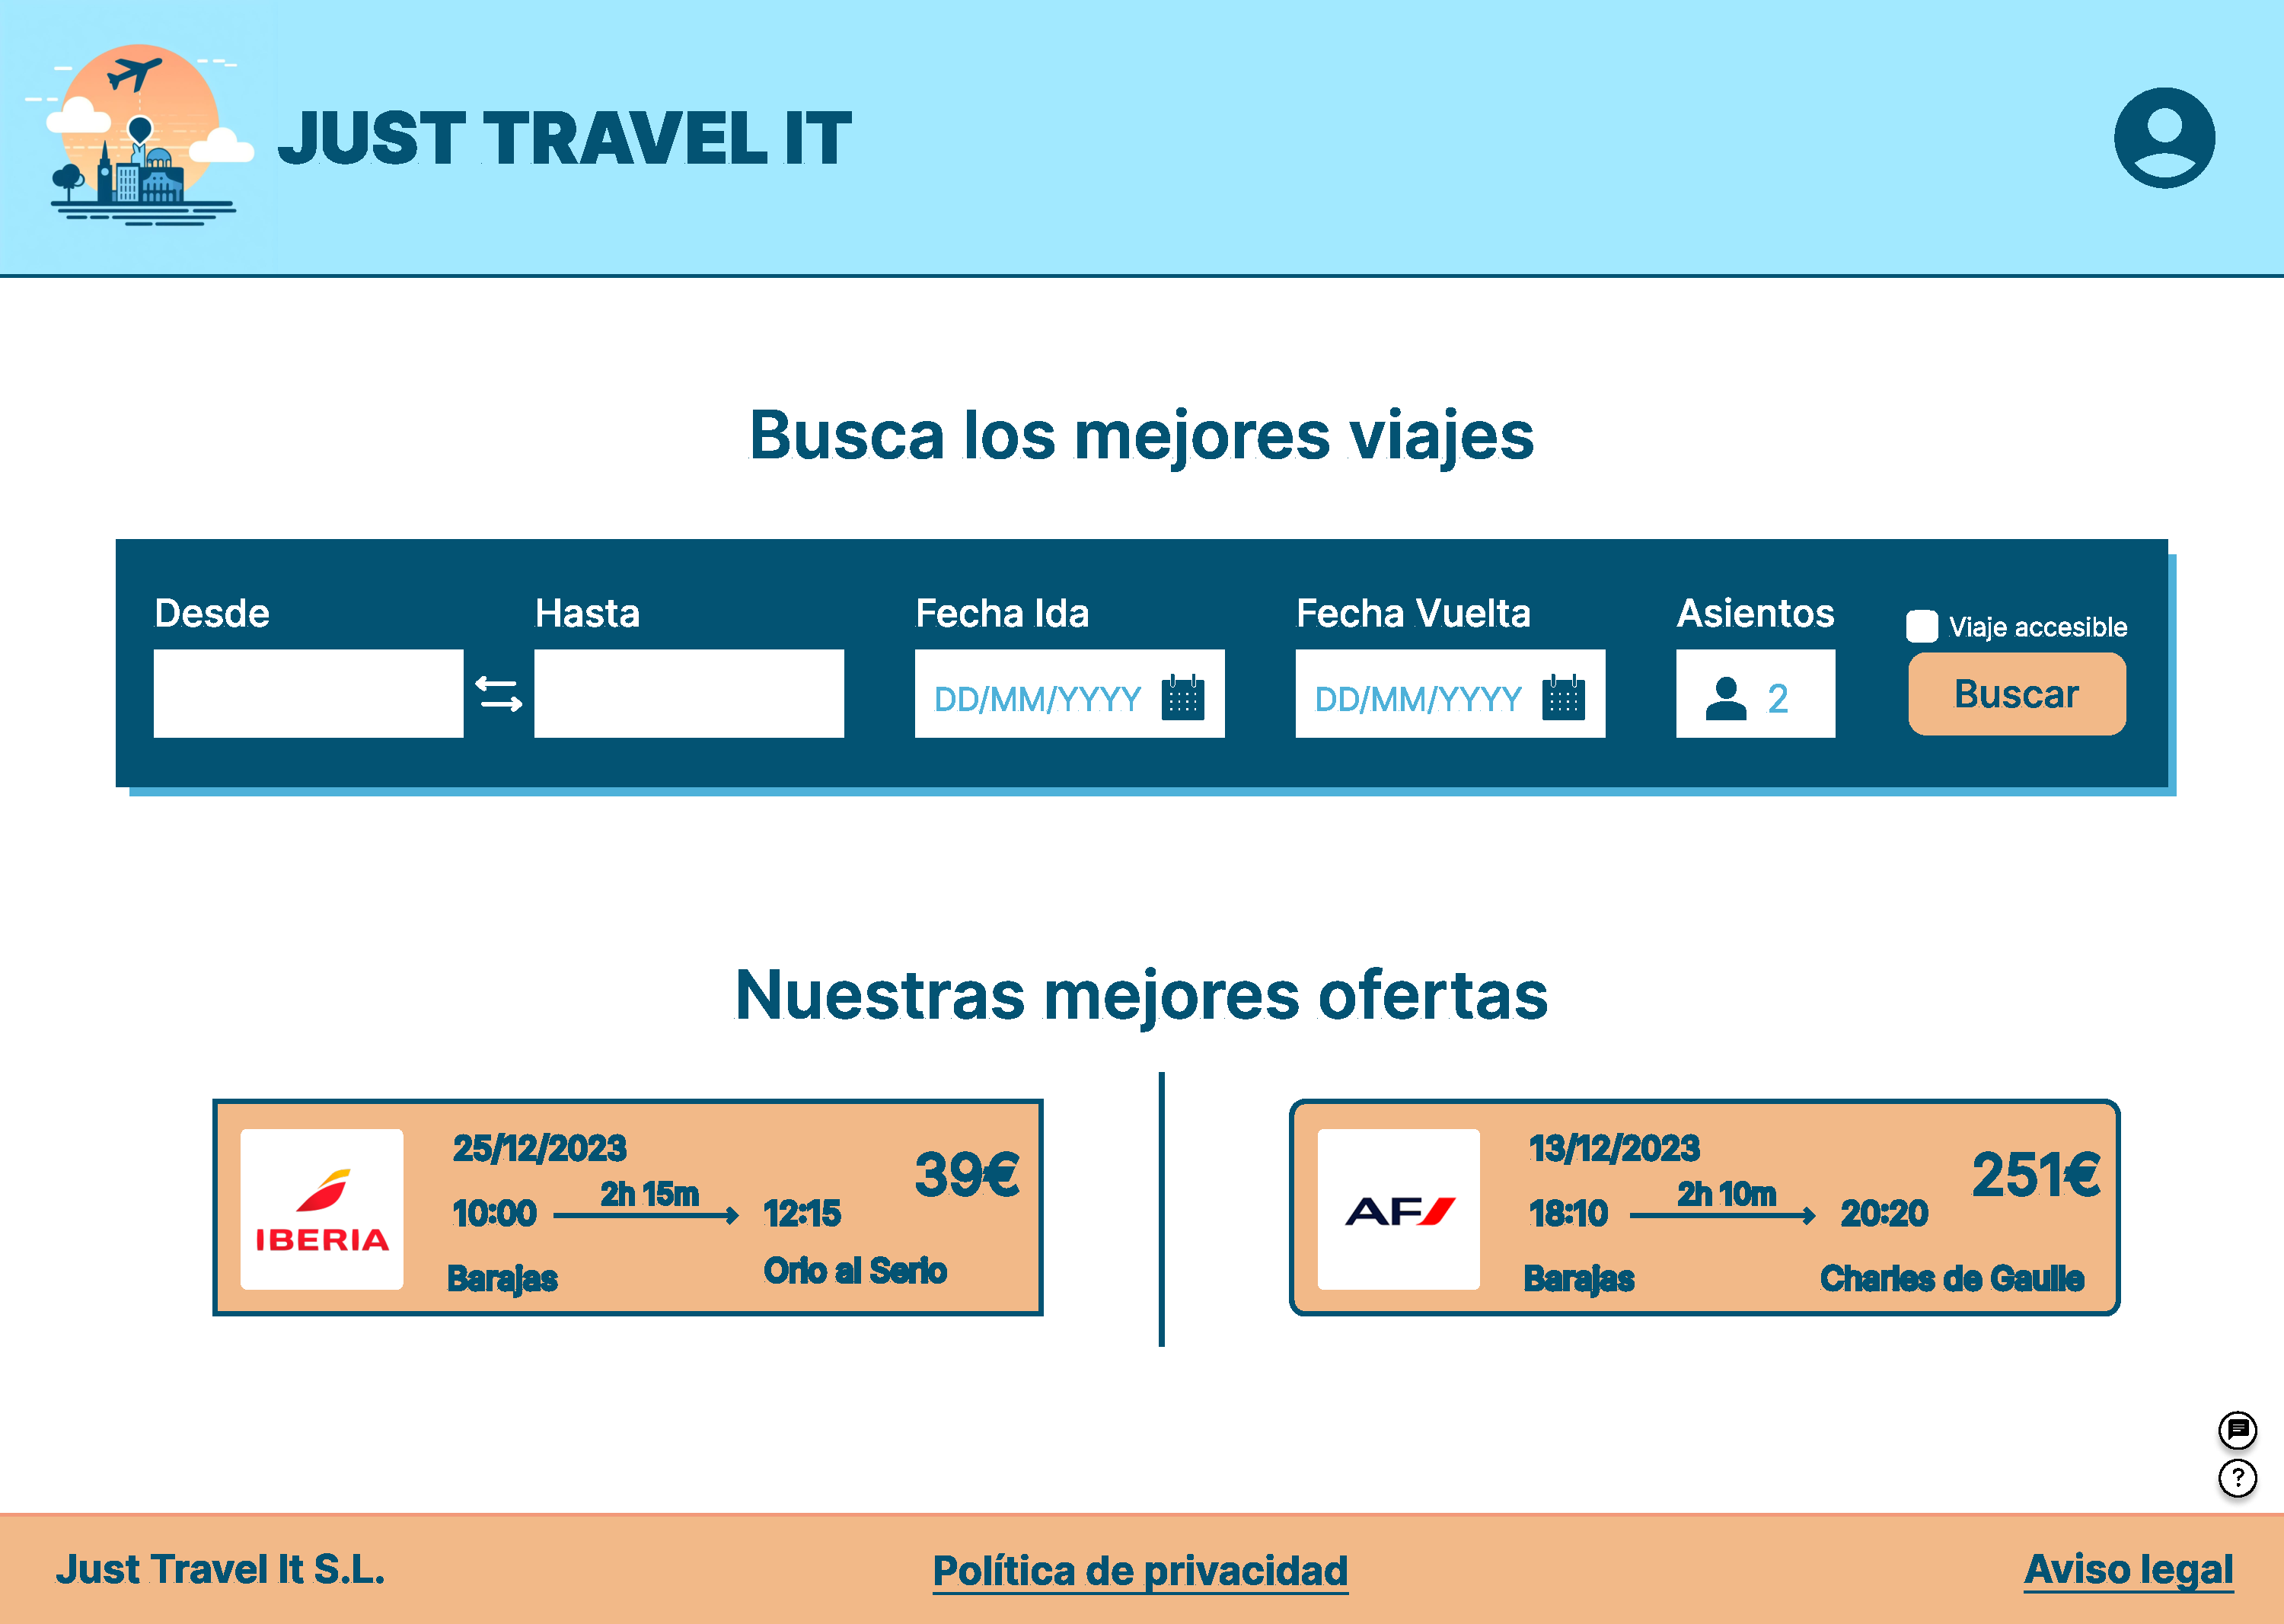
\includegraphics[page=1, width = 0.8\textwidth]{Imagenes/hito_5/it1.pdf}
    \caption{Página \textit{Inicio}}
    \label{fig:it1_inicio}
\end{figure}

\subsection{Comparador}

La pantalla del comparador (figura \ref{fig:it1_comparador}) no ha sufrido cambios con respecto al hito anterior, pero se ha cambiado el planteamiento
con respecto al hito anterior. Como ya hemos visto, dentro de la opción de búsqueda puedes seleccionar viajes
accesibles (aunque no seas una persona con discapacidad), apareciendo todos los viajes ya filtrados sin necesidad
de aplicar el filtro. Además, otra de las mejoras que se han realizado respecto a los prototipos en papel es hacer
que el botón de información de cada una de las tarjetas de los viajes muestre un \textit{pop-up} con la información más en
detalle del viaje: la información de las paradas que realiza (en caso de que las haya), la información del viaje
(la misma que se muestra en la tarjeta original), información de la compañía que opera el viaje (breve descripción
y un enlace a la página web), así como también los servicios adicionales que se ofrecen en el viaje. Se ha añadido
la funcionalidad de la ordenación de los viajes. En cuanto al contenido anterior de esta pantalla no se han realizado
modificaciones puesto que se ha considerado que la información que ya se mostraba tanto en los viajes como en los
filtros a aplicar era la necesaria. Una vez comentado el contenido de esta pantalla y las modificaciones que han
sido efectuadas, vamos a centrarnos en la identificación de los distintos patrones y principios que se han seguido
en el diseño de esta interfaz:

\begin{itemize}
    \item \textbf{Principio de proximidad.} Todas las tarjetas de los viajes de ida se encuentran bastante próximas entre
        sí y separadas de las tarjetas de viajes de vuelta, que entre sí también se encuentran cercanas, lo que
        indica que pertenecen a dos grupos distintos y claramente diferenciados. Por otro lado y aislado a este caso,
        el principio de proximidad también se aplica en el caso de las opciones de filtrado, ya que se encuentran
        todas agrupadas y próximas en la columna izquierda de la pantalla.
    \item \textbf{Consistencia interna.} al igual que ocurría con las ofertas que aparecían en la página de inicio, todas
        las tarjetas de viajes tanto de ida como de vuelta tienen la misma consistencia, puesto que la información
        que muestran y la tipografía y los colores que se utilizan son los mismos en todas las tarjetas. Otro de los
        ejemplos de la consistencia podemos observarlo en los filtros. Como puede apreciarse, aquellos filtros que se
        refieren a rangos (como el rango horario, el rango de precios o la duración), tienen el mismo formato de
        presentación, una barra en la que puedes moverte para seleccionar el filtro y unas barras que indican la
        cantidad de viajes que existen con esos valores.
    \item \textbf{Consistencia externa.} Además de la ya mencionada ubicación del botón del perfil (en la parte
        superior derecha de la pantalla), otras de las opciones que aparecen en esta pantalla y que guardan
        consistencia con la gran mayoría de las aplicaciones son los botones de Atrás y Continuar, ya que aparecen
        respectivamente en la parte izquierda y en la derecha de la aplicación, indicando la sensación de avance
        (derecha) y retroceso (izquierda).
    \item \textbf{Principio de visibilidad.} Uno de los mecanismos que tiene esta pantalla para informarte del estado de la
        misma es destacar el borde de aquellos viajes (tanto de ida como de vuelta) que hayas seleccionado, pudiendo
        conocer rápidamente las opciones que has escogido.
    \item \textbf{Ley de Hick.} Con la finalidad de no realizar un proceso de compra demasiado complejo y lleno de información,
        hemos decidido dividir el proceso en tres etapas: una primera etapa de selección de los viajes deseados,
        una segunda de datos y servicios adicionales y una tercera en la que se muestra un resumen y se procede al
        pago del viaje.
    \item \textbf{Efecto Zeigarnik.} Aunque la idea de dividir el proceso en distintas etapas se trate de un resultado de la
        Ley de Hick para intentar que sea mucho menos tedioso, la idea de mostrar la etapa del proceso en la que te
        encuentras para saber los pasos necesarios para finalizar es resultado de la aplicación directa del Efecto
        Zeigarnik.
    \item \textbf{Principio de libertad y control del usuario.} El usuario en todo momento tiene el control de la aplicación
        y puede decidir cuándo avanzar y cuándo retroceder en todo momento si ha detectado que ha cometido un error
        o bien quiere explorar otras opciones.
\end{itemize}

\begin{figure}[H]
    \centering
    \includegraphics[page=10, width = 0.8\textwidth]{Imagenes/hito_5/it1.pdf}
    \caption{Página \textit{Comparador}}
    \label{fig:it1_comparador}
\end{figure}

\subsection{Datos adicionales}

Al finalizar el proceso de selección de los viajes que se quieren reservar, la siguiente pantalla (figura \ref{fig:it1_datos_adicionales}) que aparece es
la de datos adicionales, que incluye: los datos de los pasajeros, si se desean contratar servicios
adicionales (gratuitos o bien pagando un suplemento) y la selección de los asientos. En cuanto a las modificaciones
que se han realizado con respecto al hito anterior han sido principalmente una modificación de la opción de seleccionar
asiento, ya que la información representada no era muy clara y además no mostraba información más allá de los asientos
(sólo mostraba la información de los huecos libres, sin dar información de la ubicación - filas y columnas - ni si
tenía o no ventanilla). Es por ello que se ha planificado una mejora en la que ahora se muestra una leyenda de
colores en función del estado del asiento (hemos añadido además asientos que debido a su posición dentro del vehículo
suponen un incremento del precio, por lo que se van a destacar en otro color). En cuanto a los principios de diseño que
aparecen en esta pantalla, podemos destacar los siguientes:

\begin{itemize}
    \item \textbf{Principio de cierre}. Dentro de la opción de seleccionar los datos de los pasajeros, puede verse
        cómo el campo del teléfono se encuentra entrecortado, dando la sensación a los usuarios de que puede seguir
        bajando para poder rellenar más datos.
    \item \textbf{Consistencia interna.} Las dos pestañas que se tienen para poder seleccionar los asientos y los servicios
        adicionales tienen la misma forma y tipografía, dando a entender al usuario la información contenida en
        ellas está altamente relacionada y es necesaria para poder continuar con la reserva del viaje.
    \item \textbf{Consistencia externa.} Además de la ya mencionada ubicación del botón del perfil (en la parte superior
        derecha de la pantalla), otras de las opciones que aparecen en esta pantalla y que guardan consistencia
        con la gran mayoría de las aplicaciones son los botones de Atrás y Continuar, ya que aparecen respectivamente
        en la parte izquierda y en la derecha de la aplicación, indicando la sensación de avance (derecha) y retroceso
        (izquierda).
    \item \textbf{Ley de Hick.} Con el fin de no sobrecargar la pantalla de información, los datos adicionales que se necesitan
        para la reserva se han dividido en tres secciones, de las cuales dos de ellas son desplegables, haciendo que
        la cantidad de información que se solicita al usuario puede ser regulada por él en todo momento.
    \item \textbf{Efecto Zeigarnik.} La idea de mostrar la etapa del proceso en la que te encuentras para saber los pasos
        necesarios para finalizar es resultado de la aplicación directa del Efecto Zeigarnik.
    \item \textbf{Principio de libertad y control del usuario.} El usuario en todo momento tiene el control de la aplicación
        y puede decidir cuándo avanzar y cuándo retroceder en todo momento si ha detectado que ha cometido un error
        o bien quiere explorar otras opciones.
\end{itemize}

\begin{figure}[H]
    \centering
    \includegraphics[page=11, width = 0.8\textwidth]{Imagenes/hito_5/it1.pdf}
    \caption{Página \textit{Datos adicionales}}
    \label{fig:it1_datos_adicionales}
\end{figure}

\subsection{Pago}

La última de las pantallas (figura \ref{fig:it1_pago}) necesarias para implementar la funcionalidad de realizar una reserva es la página de
pago. Una de las modificaciones realizadas (que ya mencionamos un poco anteriormente) es que antes de llegar a
esta página, si no tienes la sesión todavía iniciada, te requiere de hacerlo para poder continuar (al hacerlo te
vuelve a dirigir aquí con los datos de la compra que has realizado). En cuanto a las modificaciones realizadas
sobre la propia página, hemos mantenido la idea original de mantener los mapas de ida y de vuelta (mostrando el
itinerario a seguir) y pestañas en las que se dan dos posibles opciones de pago (tarjeta o PayPal). También
aparece el precio total del viaje, con el precio de los billetes más los suplementos que se hayan seleccionado
(servicios adicionales o asientos más caros). Sin embargo, a esto se le ha añadido un resumen de los viajes que
finalmente han sido seleccionados. Este resumen contiene las tarjetas de los viajes tanto de ida como de vuelta
y para cada una de ellas muestra la fecha, el origen, el destino y las fechas de salida y llegada. Además, cuando
se selecciona la opción de ver la información del vuelo, abre un \textit{pop-up} en el que se puede ver la información del
vuelo más detallada (los pasajeros que van a viajar, los asientos, los servicios que tiene disponibles y el precio). 

Otra de las modificaciones que se ha realizado es la información que aparece luego de confirmar la compra. En este
caso, hemos pasado de un \textit{pop-up} sencillo a una ventana en la que se muestra en detalle todo el resumen de la compra
que se ha realizado (las paradas, los destinos, las fechas, los pasajeros que van a viajar, los pasajeros y los
servicios adicionales que se han incluido en la compra). El mensaje con el número de la reserva diciendo que se ha
realizado correctamente se mantiene en la parte superior. Bajo esta información se encuentra un botón que da la
opción de continuar explorando nuevas opciones (lleva a la página de inicio). 

En cuanto a los principios de diseño que se han identificado (en ambas páginas, tanto en la referente a los datos
del pago como a la de confirmación de la compra), podemos encontrar los siguientes:

\begin{itemize}
    \item \textbf{Ley de Fitts.} Una vez decidido el método de pago con el que se va a realizar la reserva, los campos
        necesarios para efectuar la compra para cada uno de los métodos de pago se encuentran próximos entre sí
        (además de dentro de la misma pestaña), para poder facilitar al usuario moverse entre los distintos campos.
    \item \textbf{Consistencia interna.} La tipografía y los colores usados en las distintas opciones de pago (tanto en las
        pestañas como en los campos) es la misma, al igual que ocurre en el resumen de la compra (las tarjetas que
        representan los viajes de ida y de vuelta tienen la misma estructura y contienen la misma información para
        dársela al usuario). Esto también es aplicable al resumen de la compra, ya que la cantidad de información
        que se brinda en el viaje de ida es la misma que en el caso del viaje de vuelta.
    \item \textbf{Consistencia externa.} Como ya hemos visto en las etapas anteriores del proceso de reserva, se
        guarda cierta consistencia con el resto de aplicaciones, en las que se sobreentiende que el botón de retroceso
        de la página se encuentra en la parte derecha, mientras que en el caso de el de continuar (en este caso el
        botón de pagar) se encuentra en la parte derecha de la pantalla, dando la sensación de progreso.
    \item \textbf{Ley de Hick.} El número de opciones de pago que se ofrecen se encuentran separadas por pestañas,
        de modo que el usuario no se sobrecarga con una gran cantidad de información y de opciones con las que se
        puede realizar el pago.
    \item \textbf{Efecto Zeigarnik.} La idea de mostrar la etapa del proceso en la que te encuentras para saber los
        pasos necesarios para finalizar es resultado de la aplicación directa del Efecto Zeigarnik.
    \item \textbf{Principio de libertad y control del usuario.} El usuario en todo momento tiene el control de la aplicación
        y puede decidir cuándo avanzar y cuándo retroceder en todo momento si ha detectado que ha cometido un error
        o bien quiere explorar otras opciones.
    \item \textbf{Regla \textit{peak-end}.} Cuando se finaliza el proceso de reserva de la aplicación (\textit{peak}), se muestra a modo
        de finalización del proceso y para confirmar que todo se ha realizado correctamente una nueva ventana con
        un resumen de la información que se ha reservado.
\end{itemize}

\begin{figure}[H]
    \centering
    \includegraphics[page=8, width = 0.8\textwidth]{Imagenes/hito_5/it1.pdf}
    \caption{Página \textit{Pago}}
    \label{fig:it1_pago}
\end{figure}

\subsection{Inicio de sesión}

Para poder realizar reservas nuevas en la aplicación, es necesario que se inicie sesión (figura \ref{fig:it1_inicio_sesion}) con
una cuenta válida y que se encuentre ya registrada en la aplicación. Para poder realizar una
reserva completa sí que es necesario realizar el inicio de sesión, aunque para buscar viajes
no es necesario, como ya hemos visto anteriormente. Con respecto al prototipo del hito anterior
no se han realizado modificaciones aparentes sobre esta página, ya que se ha considerado que
la información que se solicita al usuario es la necesaria. En cuanto a los principios de diseño
que se han seguido para la creación de esta ventana son los siguientes:

\begin{itemize}
    \item \textbf{Ley de Fitts.} Los campos que han de rellenarse para poder iniciar sesión en la
        aplicación (correo y contraseña) se encuentran próximos entre sí, facilitando al
        usuario en todo momento el desplazamiento de uno a otro, pudiendo aportar de forma
        sencilla la información que le es solicitada.
    \item \textbf{Consistencia interna.} La tipografía y la disposición empleada para destacar los campos
        del formulario es la misma tanto en el caso del correo como en el de la contraseña (en
        la parte superior del campo se encuentra un texto que describe lo que ha de escribirse
        en el formulario y luego puede apreciarse el campo propiamente dicho).
    \item \textbf{Consistencia externa.} La página de inicio de sesión guarda consistencia externa con
        el resto de páginas de este tipo de las otras aplicaciones, ya que los campos de inicio
        de sesión se encuentran en la parte superior de la ventana, al igual que inmediatamente
        debajo de ello se encuentra el botón de iniciar sesión (si ya has rellenado los campos).
        Justo debajo de iniciar sesión, en caso de que todavía no tengas una cuenta se da la
        opción de registrarse como un nuevo usuario de la aplicación. Este ejemplo de estructura
        puede verse en el inicio de sesión de \textit{Gmail}, entre otros.
    \item \textbf{Principio de visibilidad.} Como ya vimos anteriormente, uno de los estados que va a
        manejar nuestra aplicación es el hecho de si tienes la sesión iniciada actualmente o no.
        Para poder consultar esta información, se puede observar la esquina superior derecha. Si
        el icono que aparece es el perfil, la sesión se encuentra iniciada, mientras que en el
        caso contrario, se requerirá de que se inicie sesión.
\end{itemize}

\begin{figure}[H]
    \centering
    \includegraphics[page=5, width = 0.8\textwidth]{Imagenes/hito_5/it1.pdf}
    \caption{Página \textit{Inicio de sesión}}
    \label{fig:it1_inicio_sesion}
\end{figure}

\subsection{Registro}

En el supuesto caso de que el usuario que quiera entrar a nuestra aplicación desee entrar para
poder realizar una reserva y no tenga una cuenta creada todavía, es posible darle la opción de
crearse una cuenta. Dentro de este nuevo formulario (figura \ref{fig:it1_registro}), al usuario le serán solicitados una serie
de datos adicionales (no solamente el correo y la contraseña). Estos datos adicionales han
variado con respecto al hito anterior, ya que se ha añadido nueva información para poder ofrecer
más facilidades al usuario, como por ejemplo, que a la hora de reservar un viaje, si tiene la
sesión iniciada, en los datos de los pasajeros se rellenará automáticamente la información del
primero de ellos con los datos que ya se tienen del usuario que se ha registrado en la aplicación.
En cuanto a los patrones de diseño que se han utilizado, hemos podido identificar los siguientes:


\begin{itemize}
    \item \textbf{Principio de proximidad.} Todos los campos que se necesitan para poder crear una nueva
        cuenta en la aplicación se encuentran próximos entre sí, permitiendo al usuario realizar
        movimientos muy cortos para desplazarse entre los distintos campos del registro.
    \item \textbf{Consistencia interna.} El fondo empleado tanto para cada uno de los campos así
        como la tipografía empleada para esta pantalla es consistente, ya que se mantiene dando
        una sensación de unidad en todo el conjunto de los datos.
    \item \textbf{Principio de visibilidad.} Como ya vimos anteriormente, uno de los estados que va a
        manejar nuestra aplicación es el hecho de si tienes la sesión iniciada actualmente o no.
        Para poder consultar esta información, se puede observar la esquina superior derecha. Si
        el icono que aparece es el perfil, la sesión se encuentra iniciada, mientras que en el
        caso contrario, se requerirá de que se inicie sesión.
\end{itemize}

\begin{figure}[H]
    \centering
    \includegraphics[page=2, width = 0.8\textwidth]{Imagenes/hito_5/it1.pdf}
    \caption{Página \textit{Registro}}
    \label{fig:it1_registro}
\end{figure}

\subsection{Perfil}

El usuario puede entrar a su perfil y visualizar todos los datos que haya introducido en el
registro (figura \ref{fig:it1_perfil}). Un usuario no registrado en \textit{Just Travel It} no puede acceder a esta pantalla ya que
para ello es necesario como mínimo tener un perfil en la aplicación. El usuario tampoco podrá
acceder a la pantalla de perfil si no está con sus sesión iniciada, puede ocurrir que el usuario
esté registrado pero no tenga la sesión iniciada, para ello debe iniciar sesión. En cuanto a los
principios de diseño que aparecen en esta pantalla, se pueden resaltar los siguientes:

\begin{itemize}
    \item \textbf{Consistencia interna.} El color utilizado en los botones es el mismo al igual
        que la fuente y el tamaño de la letra. No solo entre los botones dentro de la pantalla
        sino con los del resto de la aplicación.
    \item \textbf{Ley de Fitts.} La información de cada tipo se mantiene agrupada en su grupo. Los
        datos personales están todos juntos en un párrafo, mientras que la información general
        en otro, de esta forma se le facilita al usuario el encontrar la información que desee
        más ágilmente.
    \item \textbf{Ley de Hick.} Se aprovecha la clasificación del tipo de información del cliente para no
        agrupar todo en un bloque. De esta manera, evitamos que el usuario no se sobrecargue de
        información.
    \item \textbf{Principio de libertad y control del usuario.} El usuario tiene el control de su
        información en todo momento, siempre que tenga la sesión iniciada. Con esta pantalla
        tenemos el objetivo de mostrarle al usuario toda la información que ha metido en la
        aplicación y con el botón de modificar su perfil le damos la posibilidad de cambiar su
        información cuando desee.
\end{itemize}

\begin{figure}[H]
    \centering
    \includegraphics[page=12, width = 0.8\textwidth]{Imagenes/hito_5/it1.pdf}
    \caption{Página \textit{Perfil}}
    \label{fig:it1_perfil}
\end{figure}

\subsection{Modificar perfil}

Al usuario se le brinda la posibilidad de cambiar los datos de su perfil creado en \textit{Just Travel It} (figura \ref{fig:it1_mod_datos}). Podrá
modificar todos los campos rellenados en la creación del perfil. Ocurrirá lo mismo que en el \textit{Registro},
al modificar los datos, cuando se realice una reserva con la sesión iniciada se rellenaran los campos del perfil
en los campos adecuados a la reserva. Los principios empleados para la creación de esta ventana son:

\begin{itemize}
    \item \textbf{Consistencia interna.} La pantalla guarda consistencia sobre todo con la pantalla de la página de registro,
        los colores, tamaños, fuentes y tipografías se encargan de mantener la consistencia interna de estas pantallas.
    \item \textbf{Consistencia externa.} Se trata de la misma consistencia que podemos encontrar en \textit{Registro}.
    \item \textbf{Principio de proximidad.} Al ser igual que en \textit{Registro}, todas las preguntas se encuentran
        bastante próximas entre sí.
    \item \textbf{Principio de libertad y control del usuario.} El usuario en todo momento puede modificar todos
        sus datos introducidos en la aplicación.
    \item \textbf{Ley de Fitts.} Los campos que han de rellenarse para modificar el perfil se encuentran próximos
        entre sí y caben en la pantalla, por lo que no hay que hacer \textit{scroll} con el ratón, de este forma
        el usuario puede viajar con facilidad de un campo a otro.
\end{itemize}

\begin{figure}[H]
    \centering
    \includegraphics[page=4, width = 0.8\textwidth]{Imagenes/hito_5/it1.pdf}
    \caption{Página \textit{Modificar perfil}}
    \label{fig:it1_mod_datos}
\end{figure}

\subsection{Mis reservas}

Se le ofrece al usuario con una sesión iniciada que pueda consultar la información de sus reservas (figura \ref{fig:it1_reservas})
activas así como de poder comprobar las reservas pasadas. En este punto es posible consultar, modificar o cancelar
una reserva. Pasamos a nombrar los principios utilizados en esta pantalla: 

\begin{itemize}
    \item \textbf{Consistencia externa.} Al igual que en la gran mayoría de las aplicaciones, cuando el usuario
        tiene la sesión iniciada en la página, puede acceder a su perfil pulsando sobre el botón de usuario situado
        en la esquina superior derecha.
    \item \textbf{Principio de libertad y control del usuario.} El usuario en todo momento tiene el control de la
        aplicación y puede decidir cuándo avanzar y cuándo retroceder en todo momento si ha detectado que ha
        cometido un error en cuanto a la página a donde quería acceder.
    \item \textbf{Principio de visibilidad.} Como ya vimos anteriormente, uno de los estados que va a manejar
        nuestra aplicación es el hecho de si tienes la sesión iniciada actualmente o no. Para poder consultar
        esta información, se puede observar la esquina superior derecha. Si el icono que aparece es el perfil,
        la sesión se encuentra iniciada, mientras que en el caso contrario, se requerirá de que se inicie sesión. Además,
        se reconoce rápidamente la asociación ida-vuelta de los viajes.
    \item \textbf{Principio de proximidad.} Todas las tarjetas de los viajes de ida se encuentran bastante próximas entre sí
        y separadas de las tarjetas de viajes de vuelta, que entre sí también se encuentran cercanas, lo que indica
        que pertenecen a dos grupos distintos y claramente diferenciados.
\end{itemize}

\begin{figure}[H]
    \centering
    \includegraphics[page=3, width = 0.8\textwidth]{Imagenes/hito_5/it1.pdf}
    \caption{Página \textit{Mis reservas}}
    \label{fig:it1_reservas}
\end{figure}

\subsection{Consultar reserva}

Al usuario se le da la posibilidad de consultar su reserva (figura \ref{fig:it1_consulta_reserva}). Desde esta pantalla puede ver el viaje de ida y el
de vuelta, donde aparecen las tarjetas de los respectivos viajes, con las fechas, los días, la duración, la compañía,
la cantidad de pasajeros y la información adicional de la reserva. También se puede ver el mapa donde aparece la
ruta seguida en el viaje. Debajo del mapa se pueden consultar los datos de los pasajeros. Pasamos a nombrar los
principios utilizados en esta pantalla:

\begin{itemize}
    \item \textbf{Consistencia externa.} Al igual que en la gran mayoría de las aplicaciones, cuando el usuario
        tiene la sesión iniciada en la página, puede acceder a su perfil pulsando sobre el botón de usuario situado
        en la esquina superior derecha.
    \item \textbf{Consistencia interna.} La pantalla guarda consistencia sobre todo con la pantalla de la página
        resumen pago, los colores, tamaños, fuentes y tipografías se encargan de mantener la consistencia interna
        de estas pantallas.
    \item \textbf{Principio de proximidad.} Todos los campos que se necesitan para poder consultar una reserva en
        la aplicación se encuentran próximos entre sí, permitiendo al usuario realizar movimientos muy cortos para
        desplazarse entre los distintos campos.
    \item \textbf{Principio de libertad y control del usuario.} El usuario en todo momento tiene el control de la
        aplicación y puede decidir cuándo avanzar y cuándo retroceder en todo momento si ha detectado que ha cometido
        un error en cuanto a la página a dónde quería acceder.
    \item \textbf{Principio de visibilidad.} En esta pantalla se reconoce rápidamente la asociación ida-vuelta de los
        viajes.
    \item \textbf{Ley de Hick.} Con el fin de no sobrecargar la pantalla, los datos adicionales que se necesitan para
        la reserva se han dividido en dos secciones, haciendo que la cantidad de información que se muestra al
        usuario pueda ser regulada por él en todo momento.
\end{itemize}

\begin{figure}[H]
    \centering
    \includegraphics[page=6, width = 0.8\textwidth]{Imagenes/hito_5/it1.pdf}
    \caption{Página \textit{Consultar reserva}}
    \label{fig:it1_consulta_reserva}
\end{figure}


\subsection{Modificar reserva}

Al usuario se le otorga la posibilidad de modificar las reservas que haya realizado en \textit{Just Travel It} (figura \ref{fig:it1_mod_reserva}). Podrá
modificar los datos del pasajero: nombre, apellidos, DNI y teléfono. Tendrá a su disposición dos menús desplegables,
uno para poder contratar servicios adicionales que no haya contratado con anterioridad y otro en el que podrá
modificar su asiento. Además cuenta con un boton de selección en la parte inferior izquierda para poder solicitar
asistencia en la estación correspondiente por si se olvido de marcarlo a la hora de realizar la reserva. Pasamos
a nombrar los principios utilizados en esta pantalla:

\begin{itemize}
    \item \textbf{Consistencia interna.} La pantalla guarda consistencia sobre todo con la pantalla de la página
        mis reservas, los colores, tamaños, fuentes y tipografías se encargan de mantener la consistencia interna de
        estas pantallas.
    \item \textbf{Consistencia externa.} Al igual que en la gran mayoría de las aplicaciones, cuando el usuario tiene
        la sesión iniciada en la página, puede acceder a su perfil pulsando sobre el botón de usuario situado en la
        esquina superior derecha.
    \item \textbf{Ley de Fitts.} Los campos que han de rellenarse para modificar el perfil se encuentran próximos
        entre sí y caben en la pantalla, por lo que no hay que hacer \textit{scroll} con el ratón, de este forma
        el usuario puede viajar con facilidad de un campo a otro.
    \item \textbf{Principio de libertad y control del usuario.} El usuario en todo momento tiene el control de la
        aplicación y puede decidir cuándo avanzar y cuándo retroceder en todo momento si ha detectado que ha cometido
        un error en cuanto a modificar los datos.
    \item \textbf{Principio de proximidad.} Todos los campos que se necesitan para poder modificar una reserva en
        la aplicación se encuentran próximos entre sí, permitiendo al usuario realizar movimientos muy cortos para
        desplazarse entre los distintos campos a modificar.
    \item \textbf{Principio de visibilidad.} Como ya vimos anteriormente, uno de los estados que va a manejar nuestra
        aplicación es el hecho de si tienes la sesión iniciada actualmente o no. Para poder consultar esta
        información, se puede observar la esquina superior derecha. Si el icono que aparece es el perfil, la sesión
        se encuentra iniciada, mientras que en el caso contrario, se requerirá de que se inicie sesión.
\end{itemize}

\begin{figure}[H]
    \centering
    \includegraphics[page=7, width = 0.8\textwidth]{Imagenes/hito_5/it1.pdf}
    \caption{Página \textit{Modificar reserva}}
    \label{fig:it1_mod_reserva}
\end{figure}

\subsection{Soporte}

Si un usuario tiene alguna pregunta que no pueda ser abordada mediante el apartado de preguntas frecuentes previamente
mencionado (figura \ref{fig:it1_soporte}), ya sea debido a la naturaleza altamente específica de su problema o porque requiere una solución no
automatizada, o si experimenta algún inconveniente con la aplicación, tiene la opción de hacer clic en el incluíacono de
chat. Este icono se encuentra ubicado en la parte inferior derecha de cualquier pantalla de la página web, justo sobre
el icono de preguntas frecuentes.

Esta pantalla ha experimentado ciertas modificaciones con respecto al prototipo en papel. En este caso, hemos
expandido las funcionalidades de la sección de soporte, que anteriormente sólo incluía un asistente automatizado
de respuestas. La nueva sección ahora incorpora un canal de contacto telefónico, donde los usuarios pueden obtener
toda la información necesaria para comunicarse con un asistente personal. Además, hemos añadido una función de
mensajería que permite a los usuarios enviar mensajes y solicitudes directamente al equipo de asistencia al cliente,
que responderá con la mayor brevedad posible.

En cuanto a los principios de diseño que se han seguido para la creación de estas ventanas, son los siguientes:

\begin{itemize}
    \item \textbf{Principio de proximidad.} Todos los campos que se necesitan rellenar para poder enviar un nuevo
        mensaje, se encuentran próximos entre sí, permitiendo al usuario realizar movimientos muy cortos para
        desplazarse entre los distintos cuadros de texto. Relacionado a este principio, aplica la Ley de Fitts,
        donde la distancia que tiene que ser recorrida para moverse de un campo a otro es muy pequeña.
    \item \textbf{Consistencia interna.} Las distintas tarjetas que representan las formas de contactar con atención
        al cliente, tienen la misma estructura: un icono significativo, el significado de la tarjeta e información
        añadida en caso de ser necesaria. También presenta consistencia en cuanto a la forma de la tarjeta y los
        colores que se utilizan.
    \item \textbf{Consistencia externa.} Se guarda cierta consistencia con el resto de aplicaciones. Icono de
        perfil, botón de atrás y enviar, en el chat; el botón de enviar y el cuadro de texto para escribir (simulando
        el mismo que encontraríamos en un teléfono), una “X” que indica “cerrar el \textit{pop-up}”.
    \item \textbf{Feedback visual.} Una vez enviada la solicitud o mensaje al equipo de asistencia al cliente, el
        usuario recibirá un mensaje de confirmación con el objetivo de aclarar las dudas de si el mensaje ha sido
        enviado con éxito.
    \item \textbf{Principio de libertad y control del usuario.} El usuario mantiene el control total de la aplicación,
        teniendo la capacidad de avanzar o retroceder en cualquier instante. Si identifica un error o desea
        explorar alternativas, cuenta con la libertad de tomar decisiones de manera autónoma en todo momento.

\end{itemize}

\begin{figure}[H]
    \centering
    \includegraphics[page=13, width = 0.8\textwidth]{Imagenes/hito_5/it1.pdf}
    \caption{Página \textit{Soporte}}
    \label{fig:it1_soporte}
\end{figure}

\subsection{Preguntas frecuentes}

Si un usuario quiere consultar las preguntas frecuentes que pueden surgir a la hora de utilizar la aplicación,
es posible darle al botón de preguntas frecuentes marcado con una interrogación en la parte inferior derecha
de la pantalla. Esta pantalla (figura \ref{fig:it1_faq}) con respecto al prototipo en papel no ha tenido ningún cambio. Pasamos a nombrar
los principios utilizados en esta pantalla:

\begin{itemize}
    \item \textbf{Consistencia interna.} La tipografía y los colores usados en las distintas preguntas frecuentes
        es la misma, al igual que ocurre en las preguntas frecuentes desplegables. 
    \item \textbf{Consistencia externa.} Se guarda cierta consistencia con el resto de aplicaciones, empleando el
        desplegable en las preguntas para después mostrar las preguntas frecuentes relacionadas.
    \item \textbf{Principio de proximidad.} Todas las preguntas se encuentran bastante próximas entre sí.
    \item \textbf{Principio de libertad y control del usuario.} El usuario en todo momento tiene el control de la
        aplicación y puede decidir cuándo avanzar y cuándo retroceder en todo momento si ha detectado que ha cometido
        un error entrando en la pregunta que no debía o bien quiere explorar otras preguntas.
    \item \textbf{Ley de Fitts.} Los campos que han de rellenarse para modificar el perfil se encuentran próximos
        entre sí y caben en la pantalla, por lo que no hay que hacer \textit{scroll} con el ratón, de este forma el
        usuario puede viajar con facilidad de un campo a otro.
\end{itemize}

\begin{figure}[H]
    \centering
    \includegraphics[page=9, width = 0.8\textwidth]{Imagenes/hito_5/it1.pdf}
    \caption{Página \textit{Preguntas frecuentes}}
    \label{fig:it1_faq}
\end{figure}
